\section{SMT-solvers}

\subsection{School-level system of equations}

I've got this school-level system of equations copypasted from Wikipedia\footnote{\url{https://en.wikipedia.org/wiki/System_of_linear_equations}}:

\begin{alignat*}{7}
3x &&\; + \;&& 2y             &&\; - \;&& z  &&\; = \;&& 1 & \\
2x &&\; - \;&& 2y             &&\; + \;&& 4z &&\; = \;&& -2 & \\
-x &&\; + \;&& \tfrac{1}{2} y &&\; - \;&& z  &&\; = \;&& 0 &
\end{alignat*}

Will it be possible to solve it using Z3? Here it is:

\begin{lstlisting}
#!/usr/bin/python
from z3 import *

x = Real('x')
y = Real('y')
z = Real('z')
s = Solver()
s.add(3*x + 2*y - z == 1)
s.add(2*x - 2*y + 4*z == -2)
s.add(-x + 0.5*y - z == 0)
print s.check()
print s.model()
\end{lstlisting}

We see this after run:

\begin{lstlisting}
sat
[z = -2, y = -2, x = 1]
\end{lstlisting}

If we change equation in some way so it will have no solution, s.check() will return ``unsat''.

I've used ``Real'' \textit{sort} (some kind of data type in SMT-solvers) because the last expression has $\frac{1}{2}$, which is, of course, a real number.
For the integer system of equations, ``Int'' \textit{sort} would work fine.

Python (and other high-level PLs like C\#) interface is highly popular, because it's practical, but in fact, 
there is a standard language for SMT-solvers named SMT-LIB\cite{SMTLIB}.
Our example rewritten to it looks like this:

\begin{lstlisting}
(declare-const x Real)
(declare-const y Real)
(declare-const z Real)
(assert (=(-(+(* 3 x) (* 2 y)) z) 1))
(assert (=(+(-(* 2 x) (* 2 y)) (* 4 z)) -2))
(assert (=(-(+ (- 0 x) (* 0.5 y)) z) 0))
(check-sat)
(get-model)
\end{lstlisting}

This language is very close to LISP, but hard to read for untrained eyes.

Now we run it:

% FIXME:
\begin{lstlisting}
\$ z3 -smt2 example.smt
sat
(model
  (define-fun z () Real
    (- 2.0))
  (define-fun y () Real
    (- 2.0))
  (define-fun x () Real
    1.0)
)
\end{lstlisting}

So when you look back to my Python code, you may feel that these 3 expressions could be executed.
This is not true: Z3Py API offers overloaded operators, so expressions are constructed and passed into the guts of Z3 without any execution
\footnote{\url{https://github.com/Z3Prover/z3/blob/6e852762baf568af2aad1e35019fdf41189e4e12/src/api/python/z3.py}}.
I would call it ``embedded \ac{DSL}''.

% FIXME \tt, etc
Same thing for Z3 C++ API, you may find there ``operator+'' declarations and many more
\footnote{\url{https://github.com/Z3Prover/z3/blob/6e852762baf568af2aad1e35019fdf41189e4e12/src/api/c\%2B\%2B/z3\%2B\%2B.h}}.

Z3 APIs for Java, ML and .NET are also exist\footnote{\url{https://github.com/Z3Prover/z3/tree/6e852762baf568af2aad1e35019fdf41189e4e12/src/api}}.\\
\\
Z3Py tutorial: \url{https://github.com/ericpony/z3py-tutorial}.

Z3 tutorial which uses SMT-LIB language: \url{http://rise4fun.com/Z3/tutorial/guide}.

\subsection{Another school-level system of equations}

I've found this somewhere at Facebook:

\begin{figure}[H]
\centering
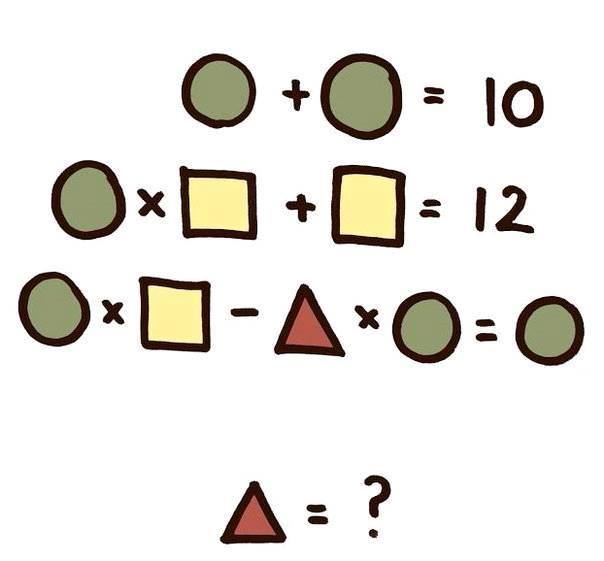
\includegraphics[scale=0.3]{SMT/equation.jpg}
\caption{System of equations}
\end{figure}

It's that easy to solve it in Z3 SMT-solver:

\begin{lstlisting}
#!/usr/bin/python
from z3 import *

circle, square, triangle = Ints('circle square triangle')
s = Solver()
s.add(circle+circle==10)
s.add(circle*square+square==12)
s.add(circle*square-triangle*circle==circle)
print s.check()
print s.model()
\end{lstlisting}

\begin{lstlisting}
sat
[triangle = 1, square = 2, circle = 5]
\end{lstlisting}

\subsection{Connection between SAT and SMT solvers}

Early SMT-solvers were frontends to SAT solvers, i.e., they translating input SMT expressions into \ac{CNF} and feed SAT-solver with it.
Conversion process is sometimes called ``bit blasting''.
Some SMT-solvers still works in that way: STP uses MiniSAT or CryptoMiniSAT as backend SAT-solver.
Some other SMT-solvers are more advanced (like Z3), so they use something even more complex.

% subsections
\subsection{Zebra puzzle (AKA Einstein puzzle)} % FIXME \ac

Zebra puzzle is a popular puzzle, defined as follows:

% FIXME remove paragraph at first line
\begin{framed}
\begin{quotation}
1.There are five houses.\\
2.The Englishman lives in the red house.\\
3.The Spaniard owns the dog.\\
4.Coffee is drunk in the green house.\\
5.The Ukrainian drinks tea.\\
6.The green house is immediately to the right of the ivory house.\\
7.The Old Gold smoker owns snails.\\
8.Kools are smoked in the yellow house.\\
9.Milk is drunk in the middle house.\\
10.The Norwegian lives in the first house.\\
11.The man who smokes Chesterfields lives in the house next to the man with the fox.\\
12.Kools are smoked in the house next to the house where the horse is kept.\\
13.The Lucky Strike smoker drinks orange juice.\\
14.The Japanese smokes Parliaments.\\
15.The Norwegian lives next to the blue house.\\
\\
Now, who drinks water? Who owns the zebra?\\
\\
In the interest of clarity, it must be added that each of the five houses is painted a different color, and their inhabitants are of different national extractions, own different pets, drink different beverages and smoke different brands of American cigarets [sic]. One other thing: in statement 6, right means your right.
\end{quotation}
\end{framed}
( \url{https://en.wikipedia.org/wiki/Zebra_Puzzle} ) \\
\\
It's a very good example of constraint satisfaction problem (CSP). % FIXME \ac

We would encode each entity as integer variable, representing number of house.

Then, to define that Englishman lives in red house, we will define this constraint: \texttt{Englishman == Red}, meaning that number of a house where Englishmen resides and where tea is drunk is the same.

To define that Norwegian lives next to the blue house, we don't realy know, if it is at left side of blue house or at right side, but we know that house numbers are different by just 1.
So we will define this constraint: \texttt{Norwegian==Blue-1 OR Norwegian==Blue+1}.

We will also need to limit all house numbers, so they will be in range of 1..5.

We will also use \texttt{Distinct} to show that all various entities of the same type are all has different house numbers.

\lstinputlisting{SMT/zebra.py}

When we run it, we got correct result:

\begin{lstlisting}
sat
[Snails = 3,
 Blue = 2,
 Ivory = 4,
 OrangeJuice = 4,
 Parliament = 5,
 Yellow = 1,
 Fox = 1,
 Zebra = 5,
 Horse = 2,
 Dog = 4,
 Tea = 2,
 Water = 1,
 Chesterfield = 2,
 Red = 3,
 Japanese = 5,
 LuckyStrike = 4,
 Norwegian = 1,
 Milk = 3,
 Kools = 1,
 OldGold = 3,
 Ukrainian = 2,
 Coffee = 5,
 Green = 5,
 Spaniard = 4,
 Englishman = 3]
 \end{lstlisting}


\subsection{Sudoku puzzle}
\label{sudoku_SMT}

Sudoku puzzle is a 9*9 grid with some cells filled, some are left to be found:

% copypasted from http://www.texample.net/tikz/examples/sudoku/
\newcounter{row}
\newcounter{col}

\newcommand\setrow[9]{
  \setcounter{col}{1}
  \foreach \n in {#1, #2, #3, #4, #5, #6, #7, #8, #9} {
    \edef\x{\value{col} - 0.5}
    \edef\y{9.5 - \value{row}}
    \node[anchor=center] at (\x, \y) {\n};
    \stepcounter{col}
  }
  \stepcounter{row}
}

\begin{center}
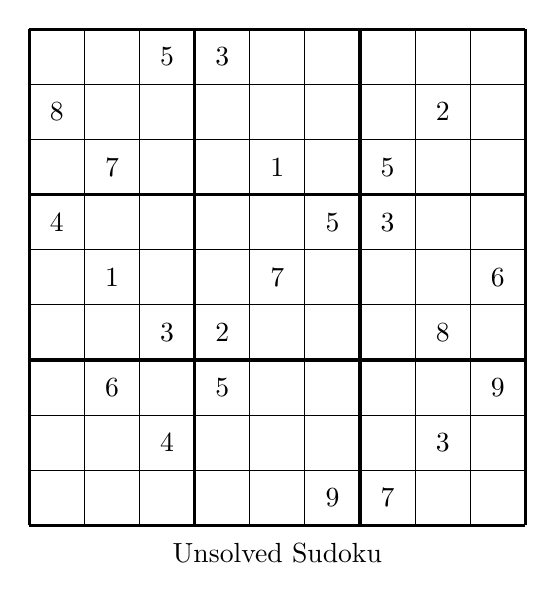
\begin{tikzpicture}[scale=.7]
  \begin{scope}
    \draw (0, 0) grid (9, 9);
    \draw[very thick, scale=3] (0, 0) grid (3, 3);

    \setcounter{row}{1}
    \setrow { }{ }{5}  {3}{ }{ }  { }{ }{ }
    \setrow {8}{ }{ }  { }{ }{ }  { }{2}{ }
    \setrow { }{7}{ }  { }{1}{ }  {5}{ }{ }

    \setrow {4}{ }{ }  { }{ }{5}  {3}{ }{ }
    \setrow { }{1}{ }  { }{7}{ }  { }{ }{6}
    \setrow { }{ }{3}  {2}{ }{ }  { }{8}{ }

    \setrow { }{6}{ }  {5}{ }{ }  { }{ }{9}
    \setrow { }{ }{4}  { }{ }{ }  { }{3}{ }
    \setrow { }{ }{ }  { }{ }{9}  {7}{ }{ }

    \node[anchor=center] at (4.5, -0.5) {Unsolved Sudoku};
  \end{scope}
\end{tikzpicture}
\end{center}

Numbers of each row must be unique, i.e., must contain all 9 numbers in range of 1..9 without repetition.
Same story for each column and also for each 3*3 square.

This puzzle is good candidate to try \ac{SMT} solver on, because it's essentially an unsolved system of equations.

\subsubsection{The first idea}

The only thing we must solve is that how to determine in one expression, if the input 9 variables has all 9 unique numbers?
They are not ordered or sorted, after all.

From the school-level mathematics, we can devise this idea:

\begin{equation}
\underbrace{10^{i_1} + 10^{i_2} + \cdots + 10^{i_9}}_9 = 1111111110
\end{equation}

Take each input variable, calculate $10^i$ and sum them all.
If all input values are unique, each will be settled at its own place.
Even more than that: there will be no holes, i.e., no skipped values.
So, in case of Sudoku, 1111111110 number will be final result, indicating that all 9 input variables are unique, in range of 1..9.

Exponentiation is heavy operation, can we use binary operations? Yes, just replace 10 with 2:

\begin{equation}
\underbrace{2^{i_1} + 2^{i_2} + \cdots + 2^{i_9}}_9 = 1111111110_2
\end{equation}

The effect is just the same, but the final value is in base 2 instead of 10.

Now a working example:

\lstinputlisting{SMT/sudoku_plus.py}
( \url{https://github.com/dennis714/SAT_SMT_article/blob/master/SMT/sudoku_plus.py} )

\begin{lstlisting}
% time python sudoku_plus.py
1 4 5 3 2 7 6 9 8
8 3 9 6 5 4 1 2 7
6 7 2 9 1 8 5 4 3
4 9 6 1 8 5 3 7 2
2 1 8 4 7 3 9 5 6
7 5 3 2 9 6 4 8 1
3 6 7 5 4 2 8 1 9
9 8 4 7 6 1 2 3 5
5 2 1 8 3 9 7 6 4

real    0m11.717s
user    0m10.896s
sys     0m0.068s
\end{lstlisting}

Even more, we can replace summing operation to logical OR:

\begin{equation}
\underbrace{2^{i_1} \vee 2^{i_2} \vee \cdots \vee 2^{i_9}}_9 = 1111111110_2
\end{equation}

% FIXME: только часть исходника
\lstinputlisting{SMT/sudoku_or.py}
( \url{https://github.com/dennis714/SAT_SMT_article/blob/master/SMT/sudoku_or.py} )

Now it works much faster. Z3 handles OR operation over bit vectors better than addition?

\begin{lstlisting}
% time python sudoku_or.py
1 4 5 3 2 7 6 9 8
8 3 9 6 5 4 1 2 7
6 7 2 9 1 8 5 4 3
4 9 6 1 8 5 3 7 2
2 1 8 4 7 3 9 5 6
7 5 3 2 9 6 4 8 1
3 6 7 5 4 2 8 1 9
9 8 4 7 6 1 2 3 5
5 2 1 8 3 9 7 6 4

real    0m1.429s
user    0m1.393s
sys     0m0.036s
\end{lstlisting}

The puzzle I used as example is dubbed as one of the hardest known
\footnote{\url{http://www.mirror.co.uk/news/weird-news/worlds-hardest-sudoku-can-you-242294}} (well, for humans).
It took \~1.4 seconds on my Intel Core i3-3110M 2.4GHz notebook to solve it.

\subsubsection{The second idea}

My first approach is far from effective, I did what first came to my mind and worked.
Another approach is to use \TT{distinct} command from SMTLIB, which tells Z3 that some variables (of unspecific number) must be distinct (or unique).
This command is also available in Z3 Python interface.

I've rewritten my first Sudoku solver, now it operates over \textit{Int} \textit{sort}, it has \TT{distinct} commands instead of bit operations,
and now also other constaint added: each cell value must be in 1..9 range, because, otherwise, Z3 will offer (although correct) solution with too big
and/or negative numbers.

% FIXME: только часть исходника
\lstinputlisting{SMT/sudoku2.py}
( \url{https://github.com/dennis714/SAT_SMT_article/blob/master/SMT/sudoku2.py} )

\begin{lstlisting}
% time python sudoku2.py
1 4 5 3 2 7 6 9 8
8 3 9 6 5 4 1 2 7
6 7 2 9 1 8 5 4 3
4 9 6 1 8 5 3 7 2
2 1 8 4 7 3 9 5 6
7 5 3 2 9 6 4 8 1
3 6 7 5 4 2 8 1 9
9 8 4 7 6 1 2 3 5
5 2 1 8 3 9 7 6 4

real    0m0.382s
user    0m0.346s
sys     0m0.036s
\end{lstlisting}

That's much faster.

\subsubsection{Conclusion}

The awesomeness of \ac{SMT}-solvers is that our Sudoku solver has nothing else, we have just defined relationships between variables (cells).

\subsubsection{Homework}

As it seems, true Sudoku puzzle is the one which has only one solution.
The piece of code I've included in this article shows only the first one.
Using the method described earlier (\ref{SMTEnumerate}, also called ``model counting''), 
try to find more solutions, or prove that the solution you have just found is the only one possible.

\subsubsection{Further reading}

\url{http://www.norvig.com/sudoku.html}

\subsubsection{Sudoku as a \ac{SAT} problem}

It's also possible to represend Sudoku puzzle as a huge \ac{CNF} equation and use \ac{SAT}-solver to find solution, but it's just trickier.

Some articles about it:
\textit{Building a Sudoku Solver with SAT}\footnote{\url{http://ocw.mit.edu/courses/electrical-engineering-and-computer-science/6-005-elements-of-software-construction-fall-2011/assignments/MIT6_005F11_ps4.pdf}},
Tjark Weber, \textit{A SAT-based Sudoku Solver}\footnote{\url{https://www.lri.fr/~conchon/mpri/weber.pdf}},
Ines Lynce, Joel Ouaknine, \textit{Sudoku as a SAT Problem}\footnote{\url{http://sat.inesc-id.pt/~ines/publications/aimath06.pdf}},
Gihwon Kwon, Himanshu Jain, \textit{Optimized CNF Encoding for Sudoku Puzzles}\footnote{\url{http://www.cs.cmu.edu/~hjain/papers/sudoku-as-SAT.pdf}}.

\ac{SMT}-solver can also use \ac{SAT}-solver in its core, so it does all mundane translating work.
As a ``compiler'', it may not do this in the most efficient way, though.


\subsection{Solving Problem Euler 31 - ``Coin sums''}

(This post was first published in my blog\footnote{\url{http://dennisyurichev.blogspot.de/2013/05/in-england-currency-is-made-up-of-pound.html}} at 10-May-2013).

\begin{framed}
\begin{quotation}
In England the currency is made up of pound, £, and pence, p, and there are eight coins in general circulation:

1p, 2p, 5p, 10p, 20p, 50p, £1 (100p) and £2 (200p).
It is possible to make £2 in the following way:

1£1 + 150p + 220p + 15p + 12p + 31p
How many different ways can £2 be made using any number of coins?
\end{quotation}
\end{framed}
( \href{http://projecteuler.net/problem=31}{Problem Euler 31 - Coin sums} )

\label{SMTEnumerate}
Using Z3 \ac{SMT} solver for solving this is overkill, and also slow, but nevertheless, it works, showing all possible solutions as well.
The piece of code for blocking already found solution and search for next, and thus, counting all solutions, was taken from Stack Overflow answer
\footnote{\url{http://stackoverflow.com/questions/11867611/z3py-checking-all-solutions-for-equation}, 
another question: \url{http://stackoverflow.com/questions/13395391/z3-finding-all-satisfying-models}}.
This is also called ``model counting''.
Constraints like ``a>=0'' must be present, because Z3 solver will search for solutions with negative numbers.

\begin{lstlisting}
#!/usr/bin/python

from z3 import *

a,b,c,d,e,f,g,h = Ints('a b c d e f g h')
s = Solver()
s.add(1*a + 2*b + 5*c + 10*d + 20*e + 50*f + 100*g + 200*h == 200, 
   a>=0, b>=0, c>=0, d>=0, e>=0, f>=0, g>=0, h>=0)
result=[]

while True:
    if s.check() == sat:
        m = s.model()
        print m
        result.append(m)
        # Create a new constraint the blocks the current model
        block = []
        for d in m:
            # d is a declaration
            if d.arity() > 0:
                raise Z3Exception("uninterpreted functions are not suppported")
            # create a constant from declaration
            c=d()
            #print c, m[d]
            if is_array(c) or c.sort().kind() == Z3_UNINTERPRETED_SORT:
                raise Z3Exception("arrays and uninterpreted sorts are not supported")
            block.append(c != m[d])
        #print "new constraint:",block
        s.add(Or(block))
    else:
        print len(result)
        break
\end{lstlisting}

Works very slow, and this is what it produces:

\begin{lstlisting}
[h = 0, g = 0, f = 0, e = 0, d = 0, c = 0, b = 0, a = 200]
[f = 1, b = 5, a = 0, d = 1, g = 1, h = 0, c = 2, e = 1]
[f = 0, b = 1, a = 153, d = 0, g = 0, h = 0, c = 1, e = 2]
...
[f = 0, b = 31, a = 33, d = 2, g = 0, h = 0, c = 17, e = 0]
[f = 0, b = 30, a = 35, d = 2, g = 0, h = 0, c = 17, e = 0]
[f = 0, b = 5, a = 50, d = 2, g = 0, h = 0, c = 24, e = 0]
\end{lstlisting}

73682 results in total.

\subsection{Using Z3 theorem prover to prove equivalence of some weird alternative to XOR operation}

(The article was first published in my blog at April 2015: \url{http://blog.yurichev.com/node/86}).

There is a "A Hacker's Assistant" program\footnote{\url{http://www.hackersdelight.org/}} (\textit{Aha!}) written by Henry Warren,
who is also the author of the great "Hacker's Delight" book.

The \textit{Aha!} program is essentially \textit{superoptimizer}\footnote{\url{http://en.wikipedia.org/wiki/Superoptimization}},
which blindly brute-force a list of some generic RISC CPU instructions to achieve shortest possible (and jumpless or branch-free) 
CPU code sequence for desired operation.
One of the impressive examples of its work is finding of Dietz's formula\footnote{\url{http://aggregate.org/MAGIC/\#Average\%20of\%20Integers}},
which is the code of computing average number of two numbers without overflow (which is important if you want to find average number of numbers like 0xFFFFFF00 and so on, using 32-bit registers).
Taking this in input:

\begin{lstlisting}
int userfun(int x, int y) {     // To find Dietz's formula for
                                // the floor-average of two
                                // unsigned integers.
   return ((unsigned long long)x + (unsigned long long)y) >> 1;
}
\end{lstlisting}

... the \textit{Aha!} gives this:

\begin{lstlisting}
Found a 4-operation program:
   and   r1,ry,rx
   xor   r2,ry,rx
   shrs  r3,r2,1
   add   r4,r3,r1
   Expr: (((y ^ x) >>s 1) + (y & x))
\end{lstlisting}

And it works correctly.

\textit{Aha!} can also find jumpless version of abs() function easily.

Compiler developers use superoptimization to find shortest possible (and/or jumpless) code, but I tried to do otherwise -- to find longest code for some basic operation.
I tried \textit{Aha!} to find equivalent of basic XOR operation without usage of the actual XOR instruction, and the most bizarre example \textit{Aha!} gave is:

\begin{lstlisting}
Found a 4-operation program:
   add   r1,ry,rx
   and   r2,ry,rx
   mul   r3,r2,-2
   add   r4,r3,r1
   Expr: (((y & x)*-2) + (y + x))
\end{lstlisting}

And it's hard to say, why/where we can use it, maybe for obfuscation, I'm not sure.
I would call this \textit{suboptimization} (as opposed to \textit{superoptimization}). Or maybe \textit{superdeoptimization}.

But my another question was also, is it possible to prove that this is correct formula at all?
The \textit{Aha!} checking some intput/output values against XOR operation, but of course, not all the possible values.
It is 32-bit code, so it may take very long time to try all possible 32-bit inputs to test it.

We can try Z3 theorem prover for the job. It's called ``prover'', after all.

So I wrote this:

\begin{lstlisting}
#!/usr/bin/python
from z3 import *

x = BitVec('x', 32)
y = BitVec('y', 32)
output = BitVec('output', 32)
s = Solver()
s.add(x^y==output)
s.add(((y & x)*0xFFFFFFFE) + (y + x)!=output)
print s.check()
\end{lstlisting}

In plain English language, this means "are there any case for x and y where $x \oplus y$ doesn't equals to $((y \& x)*-2) + (y + x)$?"
... and Z3 prints "unsat", meaning, it can't find any counterexample to the equation.
So this \textit{Aha!} output is proved to be working just like XOR operation.

Oh, I also tried to extend the formula to 64-bit:

\begin{lstlisting}
#!/usr/bin/python
from z3 import *

x = BitVec('x', 64)
y = BitVec('y', 64)
output = BitVec('output', 64)
s = Solver()
s.add(x^y==output)
s.add(((y & x)*0xFFFFFFFE) + (y + x)!=output)
print s.check()
\end{lstlisting}

Nope, now it says "sat", meaning, Z3 found at least one counterexample.
Oops, it's because I forgot to extend -2 number to 64-bit value:

\begin{lstlisting}
#!/usr/bin/python
from z3 import *

x = BitVec('x', 64)
y = BitVec('y', 64)
output = BitVec('output', 64)
s = Solver()
s.add(x^y==output)
s.add(((y & x)*0xFFFFFFFFFFFFFFFE) + (y + x)!=output)
print s.check()
\end{lstlisting}

Now it says "unsat", so the formula given by \textit{Aha!} works for 64-bit code as well.

\subsubsection{In SMT-LIB form}

Now we can rephrase our equation to more suitable form: $(x + y - ((x \& y)<<1))$.
It also works well is Z3:

\begin{lstlisting}
#!/usr/bin/python
from z3 import *

x = BitVec('x', 64)
y = BitVec('y', 64)
output = BitVec('output', 64)
s = Solver()
s.add(x^y==output)
s.add((x + y - ((x & y)<<1)) != output)
print s.check()
\end{lstlisting}

Here is how to define it in SMT-LIB way:

\begin{lstlisting}
(declare-const x (_ BitVec 64))
(declare-const y (_ BitVec 64))
(assert (not (=(bvsub (bvadd x y) (bvshl (bvand x y) (_ bv1 64))) (bvxor x y))))
(check-sat)
\end{lstlisting}

\subsubsection{Using universal quantifier}

Z3 has universal quantifier \TT{forall}, which defines a constraint, where all possible values for the equation must be true.
So we can rewrite our SMT example as:

\begin{lstlisting}
(declare-const x (_ BitVec 64))
(declare-const y (_ BitVec 64))
(forall (=(bvsub (bvadd x y) (bvshl (bvand x y) (_ bv1 64))) (bvxor x y)))
(check-sat)
\end{lstlisting}

It returns \TT{sat}, meaning, the equation is correct for all \TT{x} and \TT{y} values.

Mathematically speaking: $\forall n\!\in\!\mathbb{N}\; (x \oplus y = (x + y - ((x \& y)<<1)))$
\footnote{
$\forall$ means \textit{equation must be true for all possible values}, which are choosen from natural numbers ($\mathbb{N}$).}

\subsubsection{How the equation works}

First of all, binary addition can be viewed as binary XORing with carrying (\ref{adder}).
Here is an example: let's add 2 (10b) and 2 (10b).
XORing these two values resulting 0, but there is a carry generated during addition of two second bits.
That carry bit is propagated further and settles at the place of the 3rd bit: 100b.
4 (100b) is hence a final result of addition.

If the carry bits are not generated during addition, the addition operation is merely XORing.
For example, let's add 1 (1b) and 2 (10b). $1 + 2$ equals to 3, but $1 \oplus 2$ is also 3.

If the addition is XORing plus carry generation and application, we should eliminate effect of carrying somehow here.
The first part of the equation ($x + y$) is addition, the second ($(x \& y)<<1$) is just calculation of every carry bit which was used during addition.
Subtracting removes carry bits from the result of addition, so the only XOR effect is left then.

It's hard to say how Z3 proves this: maybe it just simplifies the equation down to single XOR using simple boolean algebra rewriting rules?


\subsection{Cracking \ac{LCG} with Z3 \ac{SMT} solver}

This part is first appeared in my blog in June 2015 at \url{http://yurichev.com/blog/modulo/}.

There are well-known weaknesses of LCG (
\href{http://en.wikipedia.org/wiki/Linear_congruential_generator#Advantages_and_disadvantages_of_LCGs}{1},
\href{http://www.reteam.org/papers/e59.pdf}{2},
\href{http://stackoverflow.com/questions/8569113/why-1103515245-is-used-in-rand/8574774#8574774}{3}
), but let's see, if it would be possible to crack it straightforwardly, without any special knowledge.
We would define all relations between LCG states in term of Z3 \ac{SMT} solver.
(I first made attempt to do it using \href{https://reference.wolfram.com/language/ref/FindInstance.html}{FindInstance} in Wolfram Mathematica, but failed, perhaps, made a mistake somewhere).
Here is a test progam:

\begin{lstlisting}
#include <stdlib.h>
#include <stdio.h>
#include <time.h>

int main()
{
	int i;

	srand(time(NULL));

	for (i=0; i<10; i++)
		printf ("%d\n", rand()%100);
};
\end{lstlisting}

It is intended to print 10 pseudorandom numbers in 0..99 range.
So it does:

\begin{lstlisting}
37
29
74
95
98
40
23
58
61
17
\end{lstlisting}

Let's say we are observing only 8 of these numbers (from 29 to 61) and we need to predict next one (17) and/or previous one (37).

The program is compiled using MSVC 2013 (I choose it because its LCG is simpler than that in Glib):

\begin{lstlisting}
.text:0040112E rand            proc near
.text:0040112E                 call    __getptd
.text:00401133                 imul    ecx, [eax+0x14], 214013
.text:0040113A                 add     ecx, 2531011
.text:00401140                 mov     [eax+14h], ecx
.text:00401143                 shr     ecx, 16
.text:00401146                 and     ecx, 7FFFh
.text:0040114C                 mov     eax, ecx
.text:0040114E                 retn
.text:0040114E rand            endp
\end{lstlisting}

This is very simple LCG, but the result is not clipped state, but it's rather shifted by 16 bits.
Let's define LCG in Z3:

\begin{lstlisting}
#!/usr/bin/python
from z3 import *

output_prev = BitVec('output_prev', 32)
state1 = BitVec('state1', 32)
state2 = BitVec('state2', 32)
state3 = BitVec('state3', 32)
state4 = BitVec('state4', 32)
state5 = BitVec('state5', 32)
state6 = BitVec('state6', 32)
state7 = BitVec('state7', 32)
state8 = BitVec('state8', 32)
state9 = BitVec('state9', 32)
state10 = BitVec('state10', 32)
output_next = BitVec('output_next', 32)

s = Solver()

s.add(state2 == state1*214013+2531011)
s.add(state3 == state2*214013+2531011)
s.add(state4 == state3*214013+2531011)
s.add(state5 == state4*214013+2531011)
s.add(state6 == state5*214013+2531011)
s.add(state7 == state6*214013+2531011)
s.add(state8 == state7*214013+2531011)
s.add(state9 == state8*214013+2531011)
s.add(state10 == state9*214013+2531011)

s.add(output_prev==URem((state1>>16)&0x7FFF,100))
s.add(URem((state2>>16)&0x7FFF,100)==29)
s.add(URem((state3>>16)&0x7FFF,100)==74)
s.add(URem((state4>>16)&0x7FFF,100)==95)
s.add(URem((state5>>16)&0x7FFF,100)==98)
s.add(URem((state6>>16)&0x7FFF,100)==40)
s.add(URem((state7>>16)&0x7FFF,100)==23)
s.add(URem((state8>>16)&0x7FFF,100)==58)
s.add(URem((state9>>16)&0x7FFF,100)==61)
s.add(output_next==URem((state10>>16)&0x7FFF,100))

print(s.check())
print(s.model())
\end{lstlisting}

URem states for \textit{unsigned remainder}.
It works for some time and gave us correct result!

\begin{lstlisting}
sat
[state3 = 2276903645,
 state4 = 1467740716,
 state5 = 3163191359,
 state7 = 4108542129,
 state8 = 2839445680,
 state2 = 998088354,
 state6 = 4214551046,
 state1 = 1791599627,
 state9 = 548002995,
 output_next = 17,
 output_prev = 37,
 state10 = 1390515370]
\end{lstlisting}

% FIXME tilde
I added ~10 states to be sure result will be correct. It may be not if you supply lesser amount of PRNG numbers.

That is the reason why LCG is not suitable for any security-related task.
This is why \href{https://en.wikipedia.org/wiki/Cryptographically_secure_pseudorandom_number_generator}{cryptographically secure pseudorandom number generators} exist: they are designed to be protected against such simple attack.
Well, at least if \href{https://en.wikipedia.org/wiki/Dual_EC_DRBG}{NSA is not involved}.

As far, as I can understand, \href{http://en.wikipedia.org/wiki/Security_token}{security tokens} like \href{http://en.wikipedia.org/wiki/RSA_SecurID}{RSA SecurID} can be viewed just as \ac{CPRNG} with a secret seed.
It shows new pseudorandom number each minute, and the server can predict it, because it knows the seed.
Imagine if such token would implement LCG -- it would be much easier to break!


\subsection{Simple hash function}

(This piece of text was initially added to my ``Reverse Engineering for Beginners'' book (\url{beginners.re}) at March 2014)
\footnote{This example was also used by Murphy Berzish in his lecture about \ac{SAT} and \ac{SMT}:
\url{http://mirror.csclub.uwaterloo.ca/csclub/mtrberzi-sat-smt-slides.pdf},
\url{http://mirror.csclub.uwaterloo.ca/csclub/mtrberzi-sat-smt.mp4}}.

Amateur cryptography is usually (unintentionally) 
very weak and can be broken easily---for cryptographers, of course.

But let's pretend we are not among these crypto-professionals.

Here is one-way hash function, that converted a 64-bit value to another and we need to try to reverse its flow back.

\subsubsection{Manual decompiling}

Here its assembly language listing in IDA:

\lstinputlisting{SMT/hash/algo_1.asm}

The example was compiled by GCC, so the first argument is passed in ECX.

If you don't have Hex-Rays, or if you distrust to it, you can try to reverse this code manually.
One method is to represent the CPU registers as local C variables and replace each instruction by a one-line equivalent expression, like:

\lstinputlisting{SMT/hash/algo_2.c}

If you are careful enough, this code can be compiled and will even work in the same way as the original.

Then, we are going to rewrite it gradually, keeping in mind all registers usage.
Attention and focus is very important here---any tiny typo may ruin all your work!

Here is the first step:

\lstinputlisting{SMT/hash/algo_3.c}

Next step:

\lstinputlisting{SMT/hash/algo_4.c}

We can spot the division using multiplication.
Indeed, let's calculate the divider in Wolfram Mathematica:

\begin{lstlisting}[caption=Wolfram Mathematica]
In[1]:=N[2^(64 + 5)/16^^8888888888888889]
Out[1]:=60.
\end{lstlisting}

We get this:

\lstinputlisting{SMT/hash/algo_5.c}

One more step:

\lstinputlisting{SMT/hash/algo_6.c}

By simple reducing, we finally see that it's calculating the remainder, not the quotient:

\lstinputlisting{SMT/hash/algo_7.c}

We end up with this fancy formatted source-code:

\lstinputlisting{SMT/hash/algo_src.c}

Since we are not cryptoanalysts we can't find an easy way to generate the input value for some specific output value.
The rotate instruction's coefficients look frightening---it's a warranty that the function is not bijective,
it has collisions, or, speaking more simply, many inputs may be possible for one output.

Brute-force is not solution because values are 64-bit ones, that's beyond reality.

\subsubsection{Now let's use the Z3 \ac{SMT} solver}

Still, without any special cryptographic knowledge, we may try to break this 
algorithm using the excellent \ac{SMT} solver from Microsoft Research named Z3\footnote{\url{http://go.yurichev.com/17314}}.
It is in fact theorem prover, but we are going to use it as \ac{SMT} solver.
Simply said, we can think about it as a system capable of solving huge equation systems.

Here is the Python source code:

\lstinputlisting[numbers=left]{SMT/hash/1.py}

This is going to be our first solver.

We see the variable definitions on line 7.
These are just 64-bit variables.
\texttt{i1..i6} are intermediate variables, representing the values in the registers between instruction executions.

Then we add the so-called constraints on lines 10..15.
The last constraint at 17 is the most important one: 
we are going to try to find an input value for which our algorithm will produce 10816636949158156260.

Essentially, the \ac{SMT}-solver searches for (any) values that satisfies all constraints.

RotateRight, RotateLeft, URem---are functions from the Z3 Python API, not related to Python language.

Then we run it:

\begin{lstlisting}
...>python.exe 1.py
sat
[i1 = 3959740824832824396,
 i3 = 8957124831728646493,
 i5 = 10816636949158156260,
 inp = 1364123924608584563,
 outp = 10816636949158156260,
 i4 = 14065440378185297801,
 i2 = 4954926323707358301]
 inp=0x12EE577B63E80B73
outp=0x961C69FF0AEFD7E4
\end{lstlisting}

``sat'' mean ``satisfiable'', i.e., the solver was able to find at least one solution.
The solution is printed in the square brackets.
The last two lines are the input/output pair in hexadecimal form.
Yes, indeed, if we run our function with \texttt{0x12EE577B63E80B73} as input, the algorithm will produce the value we were looking for.

But, as we noticed before, the function we work with is not bijective, so there may be other correct input values.
The Z3 \ac{SMT} solver is not capable of producing more than one result, but let's hack our example slightly, 
by adding line 19, which implies ``look for any other results than this'':

\lstinputlisting[numbers=left]{SMT/hash/2.py}

Indeed, it finds another correct result:

\begin{lstlisting}
...>python.exe 2.py
sat
[i1 = 3959740824832824396,
 i3 = 8957124831728646493,
 i5 = 10816636949158156260,
 inp = 10587495961463360371,
 outp = 10816636949158156260,
 i4 = 14065440378185297801,
 i2 = 4954926323707358301]
 inp=0x92EE577B63E80B73
outp=0x961C69FF0AEFD7E4
\end{lstlisting}

This can be automated.
Each found result can be added as a constraint and then the next result will be searched for.
Here is a slightly more sophisticated example:

\lstinputlisting[numbers=left]{SMT/hash/3.py}

We got:

\begin{lstlisting}
1364123924608584563
1234567890
9223372038089343698
4611686019661955794
13835058056516731602
3096040143925676201
12319412180780452009
7707726162353064105
16931098199207839913
1906652839273745429
11130024876128521237
15741710894555909141
6518338857701133333
5975809943035972467
15199181979890748275
10587495961463360371
results total= 16
\end{lstlisting}

So there are 16 correct input values for \texttt{0x92EE577B63E80B73} as a result.

The second is 1234567890---it is indeed the value which was used by me originally while preparing this example.

Let's also try to research our algorithm a bit more.
Acting on a sadistic whim, let's find if there are any possible input/output pairs in 
which the lower 32-bit parts are equal to each other?

Let's remove the \textit{outp} constraint and add another, at line 17:

\lstinputlisting[numbers=left]{SMT/hash/4.py}

It is indeed so:

\begin{lstlisting}
sat
[i1 = 14869545517796235860,
 i3 = 8388171335828825253,
 i5 = 6918262285561543945,
 inp = 1370377541658871093,
 outp = 14543180351754208565,
 i4 = 10167065714588685486,
 i2 = 5541032613289652645]
 inp=0x13048F1D12C00535
outp=0xC9D3C17A12C00535
\end{lstlisting}

Let's be more sadistic and add another constraint: last 16 bits must be \texttt{0x1234}:

\lstinputlisting[numbers=left]{SMT/hash/5.py}

Oh yes, this possible as well:

\begin{lstlisting}
sat
[i1 = 2834222860503985872,
 i3 = 2294680776671411152,
 i5 = 17492621421353821227,
 inp = 461881484695179828,
 outp = 419247225543463476,
 i4 = 2294680776671411152,
 i2 = 2834222860503985872]
 inp=0x668EEC35F961234
outp=0x5D177215F961234
\end{lstlisting}

Z3 works very fast and it implies that the algorithm is weak, it is not cryptographic at all
(like the most of the amateur cryptography).

Is it possible to tackle real cryptography by these methods? 
Real algorithms like AES, RSA, etc, can also be represented as huge system of equations, 
but these are so huge that they are impossible to work with on computers, now or in the near future.
Of course, cryptographers are fully aware of this.

Summarizing, when dealing with amateur crypto, 
it's a very good idea to try a \ac{SMT}/\ac{SAT} solver (like Z3).


\subsection{Rockey dongle: finding unknown algorithm using only input/output pairs}

(This article was first published in August 2012 in my blog: \url{http://blog.yurichev.com/node/71}).

Some smartcards can execute Java or .NET code - that's the way to hide your sensitive algorithm into chip that very hard to break (decapsulate).
For example, one may encrypt/decrypt data files by hidden crypto algorithm rendering software piracy of such software nearly impossible.

That's what called Black box in mathematics\footnote{\url{http://en.wikipedia.org/wiki/Black\_box}}.

Some software protection dongles offers this functionality too.

One example is Rockey 4 (\href{http://www.rockey.nl/en/rockey.html}{www.rockey.nl}).

\begin{figure}[H]
\centering
%\includegraphics[scale=0.66]{rockey_4.jpg}
\includegraphics[scale=2]{SMT/rockey_4.jpg}
\caption{Rockey 4 dongle}
\end{figure}

This is small dongle connected via USB. Is contain some user-defined memory but also memory for user algorithms.

The virtual (toy) CPU for these algorithms is very simple: it offer only 8 16-bit registers (however, only 4 can be set and read) and 8 operations (add, subtract, cyclic left shift, multiplication, or, xor, and, negate).

Second instruction argument can be a constant (from 0 to 63) instead of register.

Each algorithm is described by string like \colorbox{light-gray}{\TT{A=A+B, B=C*13, D=D\^{}A, C=B*55, C=C\&A, D=D|A, A=A*9, A=A\&B}}.

There are no stack, conditional/unconditional jumps, etc.

Each algorithm, obviously, can't have side effects, so they are actually pure functions
\footnote{\url{http://en.wikipedia.org/wiki/Pure_function}} and their results can be 
memoized\footnote{\url{http://en.wikipedia.org/wiki/Memoization}}.

By the way, as it was mentioned in Rockey 4 manual, first and last instruction cannot have constants. Maybe that's because these fields used for some internal data: each algorithm start and end should be marked somehow internally anyway.

Would it be possible to reveal hidden impossible-to-read algorithm only by recording input/output dongle traffic?

Common sense tell us "no". But we can try anyway.

Since, my goal wasn't to break into some Rockey-protected software, I was interesting only in limits (which algorithms could we find), so I make some things simpler: we will work with only 4 16-bit registers, and there will be only 6 operations (add, subtract, multiplication, or, xor, and).

Let's first calculate, how much information will be used in brute-force case.

There are 384 of all possible instructions in format reg=reg,op,reg for 4 registers and 6 operations, and also 6144 instructions in format reg=reg,op,constant. Remember that constant limited to 63 as maximal value? That help us for a little.

So, here 6528 all possible instructions. This mean, there are about 11854977354713530368 5-instruction algorithms. Wow! That's too much. I don't even know a precise name for such numbers. That's about 11 quintillions (thanks to Wikipedia).

Now let's try to use real heavy machinery:

\begin{framed}
\begin{quotation}
Constraint satisfaction problems (CSPs) are mathematical problems defined as a set of objects whose state must satisfy a number of constraints or limitations. CSPs represent the entities in a problem as a homogeneous collection of finite constraints over variables, which is solved by constraint satisfaction methods. CSPs are the subject of intense research in both artificial intelligence and operations research, since the regularity in their formulation provides a common basis to analyze and solve problems of many unrelated families. CSPs often exhibit high complexity, requiring a combination of heuristics and combinatorial search methods to be solved in a reasonable time. The boolean satisfiability problem (SAT), the Satisfiability Modulo Theories (SMT) and answer set programming (ASP) can be roughly thought of as certain forms of the constraint satisfaction problem.
\end{quotation}
\end{framed}\footnote{\url{http://en.wikipedia.org/wiki/Constraint_satisfaction_problem}}

... and:

\begin{framed}
\begin{quotation}
In computer science and mathematical logic, the Satisfiability Modulo Theories (SMT) problem is a decision problem for logical formulas with respect to combinations of background theories expressed in classical first-order logic with equality. Examples of theories typically used in computer science are the theory of real numbers, the theory of integers, and the theories of various data structures such as lists, arrays, bit vectors and so on. SMT can be thought of as a form of the constraint satisfaction problem and thus a certain formalized approach to constraint programming.
\end{quotation}
\end{framed}\footnote{\url{http://en.wikipedia.org/wiki/Satisfiability_Modulo_Theories}}

I'll use Z3 Theorem Prover
\footnote{\url{http://research.microsoft.com/en-us/um/redmond/projects/z3/}} from Microsoft Research with excellent 
Python bindings, working like SMT solver.

It can be said, SMT solver is just solver of very big system of equations. 
By the way, its sibling SAT solver is intended for solving very big boolean system of equations.

Needless to say, a lot of tasks can be expressed as system of equations. 
One very simple example is Sudoku: \url{https://sites.google.com/site/modante/sudokusolver}

So let's back to our toy CPU inside of Rockey 4 dongle.

How can we express each instruction as system of equations? While remembering some school math, I wrote this:

% WAT THIS IS?
Function one\_step()=

\begin{lstlisting}
Each Bx is integer, but may be only 0 or 1.

# only one of B1..B4 and B5..B9 can be set
reg1=B1*A + B2*B + B3*C + B4*D
reg_or_constant2=B5*A + B6*B + B7*C + B8*D + B9*constant
reg1 should not be equal to reg_or_constant2

# Only one of B10..B15, can be set
result=result+B10*(reg1*reg2)
result=result+B11*(reg1^reg2)
result=result+B12*(reg1+reg2)
result=result+B13*(reg1-reg2)
result=result+B14*(reg1|reg2)
result=result+B15*(reg1&reg2)

B16 - true if register isn't updated in this part
B17 - true if register is updated in this part
(B16 cannot be equal to B17)
A=B16*A + B17*result
B=B18*A + B19*result
C=B20*A + B21*result
D=B22*A + B23*result
\end{lstlisting}

That's how we can express each instruction in algorithm.

5-instructions algorithm can be expressed like this: one\_step (one\_step (one\_step (one\_step (one\_step (input\_registers)))))

Let's also add five known input/output pairs and we'll get system of equations like this:

\begin{lstlisting}
one_step (one_step (one_step (one_step (one_step (input_1)))))==output_1
one_step (one_step (one_step (one_step (one_step (input_2)))))==output_2
one_step (one_step (one_step (one_step (one_step (input_3)))))==output_3
one_step (one_step (one_step (one_step (one_step (input_4)))))==output_4
.. etc
\end{lstlisting}

So the question now is to find about 5*23 boolean values satisfying known input/output pairs.

I wrote small utility to probe Rockey 4 algorithm with random numbers, it produce results in form:

\begin{lstlisting}
RY_CALCULATE1: (input) p1=30760 p2=18484 p3=41200 p4=61741 (output) p1=49244 p2=11312 p3=27587 p4=12657
RY_CALCULATE1: (input) p1=51139 p2=7852 p3=53038 p4=49378 (output) p1=58991 p2=34134 p3=40662 p4=9869
RY_CALCULATE1: (input) p1=60086 p2=52001 p3=13352 p4=45313 (output) p1=46551 p2=42504 p3=61472 p4=1238
RY_CALCULATE1: (input) p1=48318 p2=6531 p3=51997 p4=30907 (output) p1=54849 p2=20601 p3=31271 p4=44794
\end{lstlisting}

p1/p2/p3/p4 are just another names for A/B/C/D registers.

Now let's start with Z3. We will need to express Rockey 4 toy CPU in Z3Py (Z3 for Python) terms.

It can be said, my Python script is divided into two parts: 

\begin{itemize}
\item
constraint definitions (like, "output\_1 should be n for input\_1=m", "constant cannot be greater than 64", etc); 

\item
functions constructing system of equations.
\end{itemize}

This piece of code define some kind of "structure" consisting of 4 named 16-bit variables, each represent register in our toy CPU.

\begin{lstlisting}
Registers_State=Datatype ('Registers_State')
Registers_State.declare('cons', ('A', BitVecSort(16)), ('B', BitVecSort(16)), ('C', BitVecSort(16)), ('D', BitVecSort(16)))
Registers_State=Registers_State.create()
\end{lstlisting}

These enumarations define two new types (or "sorts" in Z3's terminology):

\begin{lstlisting}
Operation, (OP_MULT, OP_MINUS, OP_PLUS, OP_XOR, OP_OR, OP_AND) = EnumSort('Operation', ('OP_MULT', 'OP_MINUS', 'OP_PLUS', 'OP_XOR', 'OP_OR', 'OP_AND'))

Register, (A, B, C, D) = EnumSort('Register', ('A', 'B', 'C', 'D'))
\end{lstlisting}

This part is very important, it define all variables in our system of equations. 
op\_step is type of operation in instruction. reg\_or\_constant is selector between register or constant in second 
argument --- False if register and True if constant. 
reg\_step is register assigned in this instruction. 
reg1\_step and reg2\_step are just registers at arg1 and arg2. 
constant\_step is constant (in case it's used in instruction instead of arg2).

\begin{lstlisting}
op_step=[Const('op_step%s' % i, Operation) for i in range(STEPS)]
reg_or_constant_step=[Bool('reg_or_constant_step%s' % i) for i in range(STEPS)]
reg_step=[Const('reg_step%s' % i, Register) for i in range(STEPS)]
reg1_step=[Const('reg1_step%s' % i, Register) for i in range(STEPS)]
reg2_step=[Const('reg2_step%s' % i, Register) for i in range(STEPS)]
constant_step = [BitVec('constant_step%s' % i, 16) for i in range(STEPS)]
\end{lstlisting}

Adding constraints is very simple. Remember, I wrote that each constant cannot be larger than 63?

\begin{lstlisting}
# according to Rockey 4 dongle manual, arg2 in first and last instructions cannot be a constant
s.add (reg_or_constant_step[0]==False)
s.add (reg_or_constant_step[STEPS-1]==False)

...

for x in range(STEPS):
   s.add (constant_step[x]>=0, constant_step[x]<=63)
\end{lstlisting}

Input/output values are added as constraints too.

Now let's see how to construct our system of equations:

\begin{lstlisting}
# Register, Registers_State -> int
def register_selector (register, input_registers):
    return If(register==A, Registers_State.A(input_registers),
           If(register==B, Registers_State.B(input_registers), 
           If(register==C, Registers_State.C(input_registers), 
           If(register==D, Registers_State.D(input_registers), 
                           0)))) # default
\end{lstlisting}

This function returning corresponding register value from "structure". 
Needless to say, the code above is not executed. 
If() is Z3Py function. 
The code only declares the function, which will be used in another. 
By the way, expression declaration resembling LISP language in some way.

Here is another function where register\_selector() used:

\begin{lstlisting}
# Bool, Register, Registers_State, int -> int
def register_or_constant_selector (register_or_constant, register, input_registers, constant): 
    return If(register_or_constant==False, register_selector(register, input_registers), constant)
\end{lstlisting}

The code here is never executed too. 
It only construct one small piece of very big expression. 
But for the sake of simplicity, one can think all these functions will be called during bruteforce search.

\begin{lstlisting}
# Operation, Bool, Register, Register, Int, Registers_State -> int
def one_op (op, register_or_constant, reg1, reg2, constant, input_registers):
    arg1=register_selector(reg1, input_registers)
    arg2=register_or_constant_selector (register_or_constant, reg2, input_registers, constant)
    return If(op==OP_MULT,   arg1*arg2,
           If(op==OP_MINUS,  arg1-arg2,
           If(op==OP_PLUS,   arg1+arg2, 
           If(op==OP_XOR,    arg1^arg2, 
           If(op==OP_OR,     arg1|arg2, 
           If(op==OP_AND,    arg1&arg2, 
                          0)))))) # default
\end{lstlisting}

Here is expression describing each instruction. 
Register assigned is instruction is substitued with new\_val, 
while all other registers are copied from input register's state:

\begin{lstlisting}
# Bool, Register, Operation, Register, Register, Int, Registers_State -> Registers_State
def one_step (register_or_constant, register_assigned_in_this_step, op, reg1, reg2, constant, input_registers):
    new_val=one_op(op, register_or_constant, reg1, reg2, constant, input_registers)
    return If (register_assigned_in_this_step==A, Registers_State.cons (new_val,
                                                                        Registers_State.B(input_registers), 
                                                                        Registers_State.C(input_registers), 
                                                                        Registers_State.D(input_registers)),
           If (register_assigned_in_this_step==B, Registers_State.cons (Registers_State.A(input_registers), 
                                                                        new_val,
                                                                        Registers_State.C(input_registers),
                                                                        Registers_State.D(input_registers)), 
           If (register_assigned_in_this_step==C, Registers_State.cons (Registers_State.A(input_registers), 
                                                                        Registers_State.B(input_registers), 
                                                                        new_val,
                                                                        Registers_State.D(input_registers)), 
           If (register_assigned_in_this_step==D, Registers_State.cons (Registers_State.A(input_registers), 
                                                                        Registers_State.B(input_registers), 
                                                                        Registers_State.C(input_registers), 
                                                                        new_val),
                                                  Registers_State.cons(0,0,0,0))))) # default
\end{lstlisting}

This is the last function describing whole n-step program:

\begin{lstlisting}
def program(input_registers, STEPS):
    cur_input=input_registers
    for x in range(STEPS):
        cur_input=one_step (reg_or_constant_step[x], reg_step[x], op_step[x], reg1_step[x], reg2_step[x], constant_step[x], cur_input)
    return cur_input
\end{lstlisting}

Again, for the sake of simplicity, it can be said, now Z3 will try each possible registers/operations/constants against this expression to find such combination which satisfy input/output pairs. 
But it's not true. 
As far as I right, Z3 use DPLL algorithm\footnote{\url{http://en.wikipedia.org/wiki/DPLL_algorithm}}.

Now let's start with very simple 3-step algorithm: "B=A\^{}D, C=D*D, D=A*C". Please note: register A left unchanged.
I programmed Rockey 4 dongle with it and recorded algorithm outputs:

\begin{lstlisting}
RY_CALCULATE1: (input) p1=8803 p2=59946 p3=36002 p4=44743 (output) p1=8803 p2=36004 p3=7857 p4=24691
RY_CALCULATE1: (input) p1=5814 p2=55512 p3=52155 p4=55813 (output) p1=5814 p2=52403 p3=33817 p4=4038
RY_CALCULATE1: (input) p1=25206 p2=2097 p3=55906 p4=22705 (output) p1=25206 p2=15047 p3=10849 p4=43702
RY_CALCULATE1: (input) p1=10044 p2=14647 p3=27923 p4=7325 (output) p1=10044 p2=15265 p3=47177 p4=20508
RY_CALCULATE1: (input) p1=15267 p2=2690 p3=47355 p4=56073 (output) p1=15267 p2=57514 p3=26193 p4=53395
\end{lstlisting}

It took about one second and only 5 pairs above to find algorithm (on my quad-core Xeon E3-1220 (clocked at 3.1GHz), 
however, Z3 solver working in single-thread mode):

\begin{lstlisting}
B = A ^ D
C = D * D
D = C * A
\end{lstlisting}

Notice last instruction: C and A registers are swapped comparing to version I wrote by hand. 
But of course, this instruction is working in the same way.

Now if I try to find all 4-step programs satisfying to these values, my script will offer this:

\begin{lstlisting}
B = A ^ D
C = D * D
D = A * C
A = A | A
\end{lstlisting}

... and that's really fun, because last instruction do nothing with value in register A, it's like "no operation" 
--- but still, algorithm is correct for values given!

Here is another 5-step algorithm: "B=B\^{}D, C=A*22, A=B*19, A=A\&42, D=B\&C" and values:

\begin{lstlisting}
RY_CALCULATE1: (input) p1=61876 p2=28737 p3=28636 p4=50362 (output) p1=32 p2=46331 p3=50552 p4=33912
RY_CALCULATE1: (input) p1=46843 p2=43355 p3=39078 p4=24552 (output) p1=8 p2=63155 p3=47506 p4=45202
RY_CALCULATE1: (input) p1=22425 p2=51432 p3=40836 p4=14260 (output) p1=0 p2=65372 p3=34598 p4=34564
RY_CALCULATE1: (input) p1=44214 p2=45766 p3=19778 p4=59924 (output) p1=2 p2=22738 p3=55204 p4=20608
RY_CALCULATE1: (input) p1=27348 p2=49060 p3=31736 p4=59576 (output) p1=0 p2=22300 p3=11832 p4=1560
\end{lstlisting}

It took 37 seconds and we've got:

\begin{lstlisting}
B = D ^ B
C = A * 22
A = B * 19
A = A & 42
D = C & B
\end{lstlisting}

A=A\&42 was correctly deduced (look at these five p1's at output (assigned to output A register): 32,8,0,2,0)

6-step algorithm "A=A+B, B=C*13, D=D\^{}A, C=C\&A, D=D|B, A=A\&B" and values:

\begin{lstlisting}
RY_CALCULATE1: (input) p1=4110 p2=35411 p3=54308 p4=47077 (output) p1=32832 p2=50644 p3=36896 p4=60884
RY_CALCULATE1: (input) p1=12038 p2=7312 p3=39626 p4=47017 (output) p1=18434 p2=56386 p3=2690 p4=64639
RY_CALCULATE1: (input) p1=48763 p2=27663 p3=12485 p4=20563 (output) p1=10752 p2=31233 p3=8320 p4=31449
RY_CALCULATE1: (input) p1=33174 p2=38937 p3=54005 p4=38871 (output) p1=4129 p2=46705 p3=4261 p4=48761
RY_CALCULATE1: (input) p1=46587 p2=36275 p3=6090 p4=63976 (output) p1=258 p2=13634 p3=906 p4=48966
\end{lstlisting}

90 seconds and we've got:

\begin{lstlisting}
A = A + B
B = C * 13
D = D ^ A
D = B | D
C = C & A
A = B & A
\end{lstlisting}

But that was simple, however. 
Some tasks are not possible even for 6-step algorithms, for example: "A=A\^{}B, A=A*9, A=A\^{}C, A=A*19, A=A\^{}D, A=A\&B".
Solver was working too long (up to several hours), so I didn't even know is it possible to find it anyway.\\

\subsubsection{Conclusion}

This is in fact an exercise in program synthesis.

Some short algorithms for tiny CPU's are really possible to find using so minimum data about it! 
Of course it's still not possible to reveal some harder algorithm, but this method definitely should not be ignored!

Now, files: Rockey 4 dongle programmer and reader, Rockey 4 manual, Z3Py script for finding algorithms, input/output pairs, and also fixed z3.py file from Z3 (my script may fail to work with unfixed z3.py coming with Z3 4.0 installation, so I got another, you may try to use it too):

\url{http://yurichev.com/non-wiki-files/rockey4_algo_search.zip}

\subsubsection{Future work}

Perhaps, constructing LISP-like S-expression can be better than a program for toy-level CPU.

It's also possible to start with smaller constants and then proceed to bigger.
This is somewhat similar to increasing password length in password brute-force cracking.



